
\documentclass[12pt]{beamer}
\usepackage{amsmath}
\usepackage{mathtools}
\usepackage{multimedia}
\usepackage{hyperref}


\usefonttheme{professionalfonts} % using non standard fonts for beamer
\usefonttheme{serif} % default family is serif
%\documentclass[12pt]{beamerthemeSam.sty}
\usepackage{epsf}
%\usepackage{pstricks}
%\usepackage[orientation=portrait,size=A4]{beamerposter}
\geometry{paperwidth=160mm,paperheight=120mm}
%DT favorite definitions
\def\LL{\left\langle}	% left angle bracket
\def\RR{\right\rangle}	% right angle bracket
\def\LP{\left(}		% left parenthesis
\def\RP{\right)}	% right parenthesis
\def\LB{\left\{}	% left curly bracket
\def\RB{\right\}}	% right curly bracket
\def\PAR#1#2{ {{\partial #1}\over{\partial #2}} }
\def\PARTWO#1#2{ {{\partial^2 #1}\over{\partial #2}^2} }
\def\PARTWOMIX#1#2#3{ {{\partial^2 #1}\over{\partial #2 \partial #3}} }

\def\rightpartial{{\overrightarrow\partial}}
\def\leftpartial{{\overleftarrow\partial}}
\def\diffpartial{\buildrel\leftrightarrow\over\partial}

\def\BCC{\begin{columns}}
\def\ECC{\end{columns}}
\def\HC {\column{0.5\textwidth}}

\def\BC{\begin{center}}
\def\EC{\end{center}}
\def\BN{\begin{enumerate}}
\def\EN{\end{enumerate}}
\def\BI{\begin{itemize}}
\def\EI{\end{itemize}}
\def\BE{\begin{displaymath}}
\def\EE{\end{displaymath}}
\def\BEA{\begin{eqnarray*}}
\def\EEA{\end{eqnarray*}}
\def\BNEA{\begin{eqnarray}}
\def\ENEA{\end{eqnarray}}
\def\EL{\nonumber\\}

\newcommand{\etal}{{\it et al.}}
\newcommand{\gbeta}{6/g^2}
\newcommand{\la}[1]{\label{#1}}
\newcommand{\ie}{{\em i.e.\ }}
\newcommand{\eg}{{\em e.\,g.\ }}
\newcommand{\cf}{cf.\ }
\newcommand{\BS}{\bigskip}
\newcommand{\etc}{etc.\ }
\newcommand{\atantwo}{{\rm atan2}}
\newcommand{\Tr}{{\rm Tr}}
\newcommand{\dt}{\Delta t}
\newcommand{\op}{{\cal O}}
\newcommand{\msbar}{{\overline{\rm MS}}}
\def\chpt{\raise0.4ex\hbox{$\chi$}PT}
\def\schpt{S\raise0.4ex\hbox{$\chi$}PT}
\def\MeV{{\rm Me\!V}}
\def\GeV{{\rm Ge\!V}}

%AB: my color definitions
%\definecolor{mygarnet}{rgb}{0.445,0.184,0.215}
%\definecolor{mygold}{rgb}{0.848,0.848,0.098}
%\definecolor{myg2g}{rgb}{0.647,0.316,0.157}
\definecolor{A}{rgb}{1.0,0.3,0.3}
\definecolor{B}{rgb}{0.0,1.0,0.0}
\definecolor{C}{rgb}{1.0,1.0,0.0}
\definecolor{D}{rgb}{0.5,0.5,1.0}
\definecolor{E}{rgb}{0.7,0.7,0.7}
\definecolor{abtitlecolor}{rgb}{1.0,1.0,1.0}
\definecolor{absecondarycolor}{rgb}{0.0,0.416,0.804}
\definecolor{abprimarycolor}{rgb}{1.0,0.686,0.0}
\definecolor{Red}           {rgb}{1,0.4,0.4}
\definecolor{Yellow}           {rgb}{1,1,0.0}
\definecolor{Grey}          {cmyk}{.7,.7,.7,0}
\definecolor{Blue}          {cmyk}{1,1,0,0}
\definecolor{Green}         {cmyk}{1,0,1,0}
\definecolor{Brown}         {cmyk}{0,0.81,1,0.60}
\definecolor{Silver}        {rgb}{0.95,0.9,1.0}
\definecolor{Sky}           {rgb}{0.07,0.0,0.2}
\definecolor{Darkbrown}     {rgb}{0.4,0.3,0.2}
\definecolor{Black}         {rgb}{0.0,0.0,0.0}
\definecolor{40Gray}        {rgb}{0.4,0.4,0.5}
\usetheme{Madrid}


\setbeamercolor{normal text}{fg=Silver,bg=Sky}

%AB: redefinition of beamer colors
%\setbeamercolor{palette tertiary}{fg=white,bg=mygarnet}
%\setbeamercolor{palette secondary}{fg=white,bg=myg2g}
%\setbeamercolor{palette primary}{fg=black,bg=mygold}
\setbeamercolor{title}{fg=abtitlecolor}
\setbeamercolor{frametitle}{fg=abtitlecolor}
\setbeamercolor{palette tertiary}{fg=white,bg=Darkbrown}
\setbeamercolor{palette secondary}{fg=white,bg=absecondarycolor}
\setbeamercolor{palette primary}{fg=white,bg=40Gray}
\setbeamercolor{structure}{fg=abtitlecolor}

\setbeamerfont{section in toc}{series=\bfseries}

%AB: remove navigation icons
\beamertemplatenavigationsymbolsempty
\title[Thermal radiation]{
  \textbf {Thermal radiation and spectroscopy}}

\author [Astronomy 101]{Astronomy 101\\Syracuse University, Fall 2022\\Walter Freeman}

\date{\today}

\begin{document}



\frame{\titlepage}

\frame{
\BC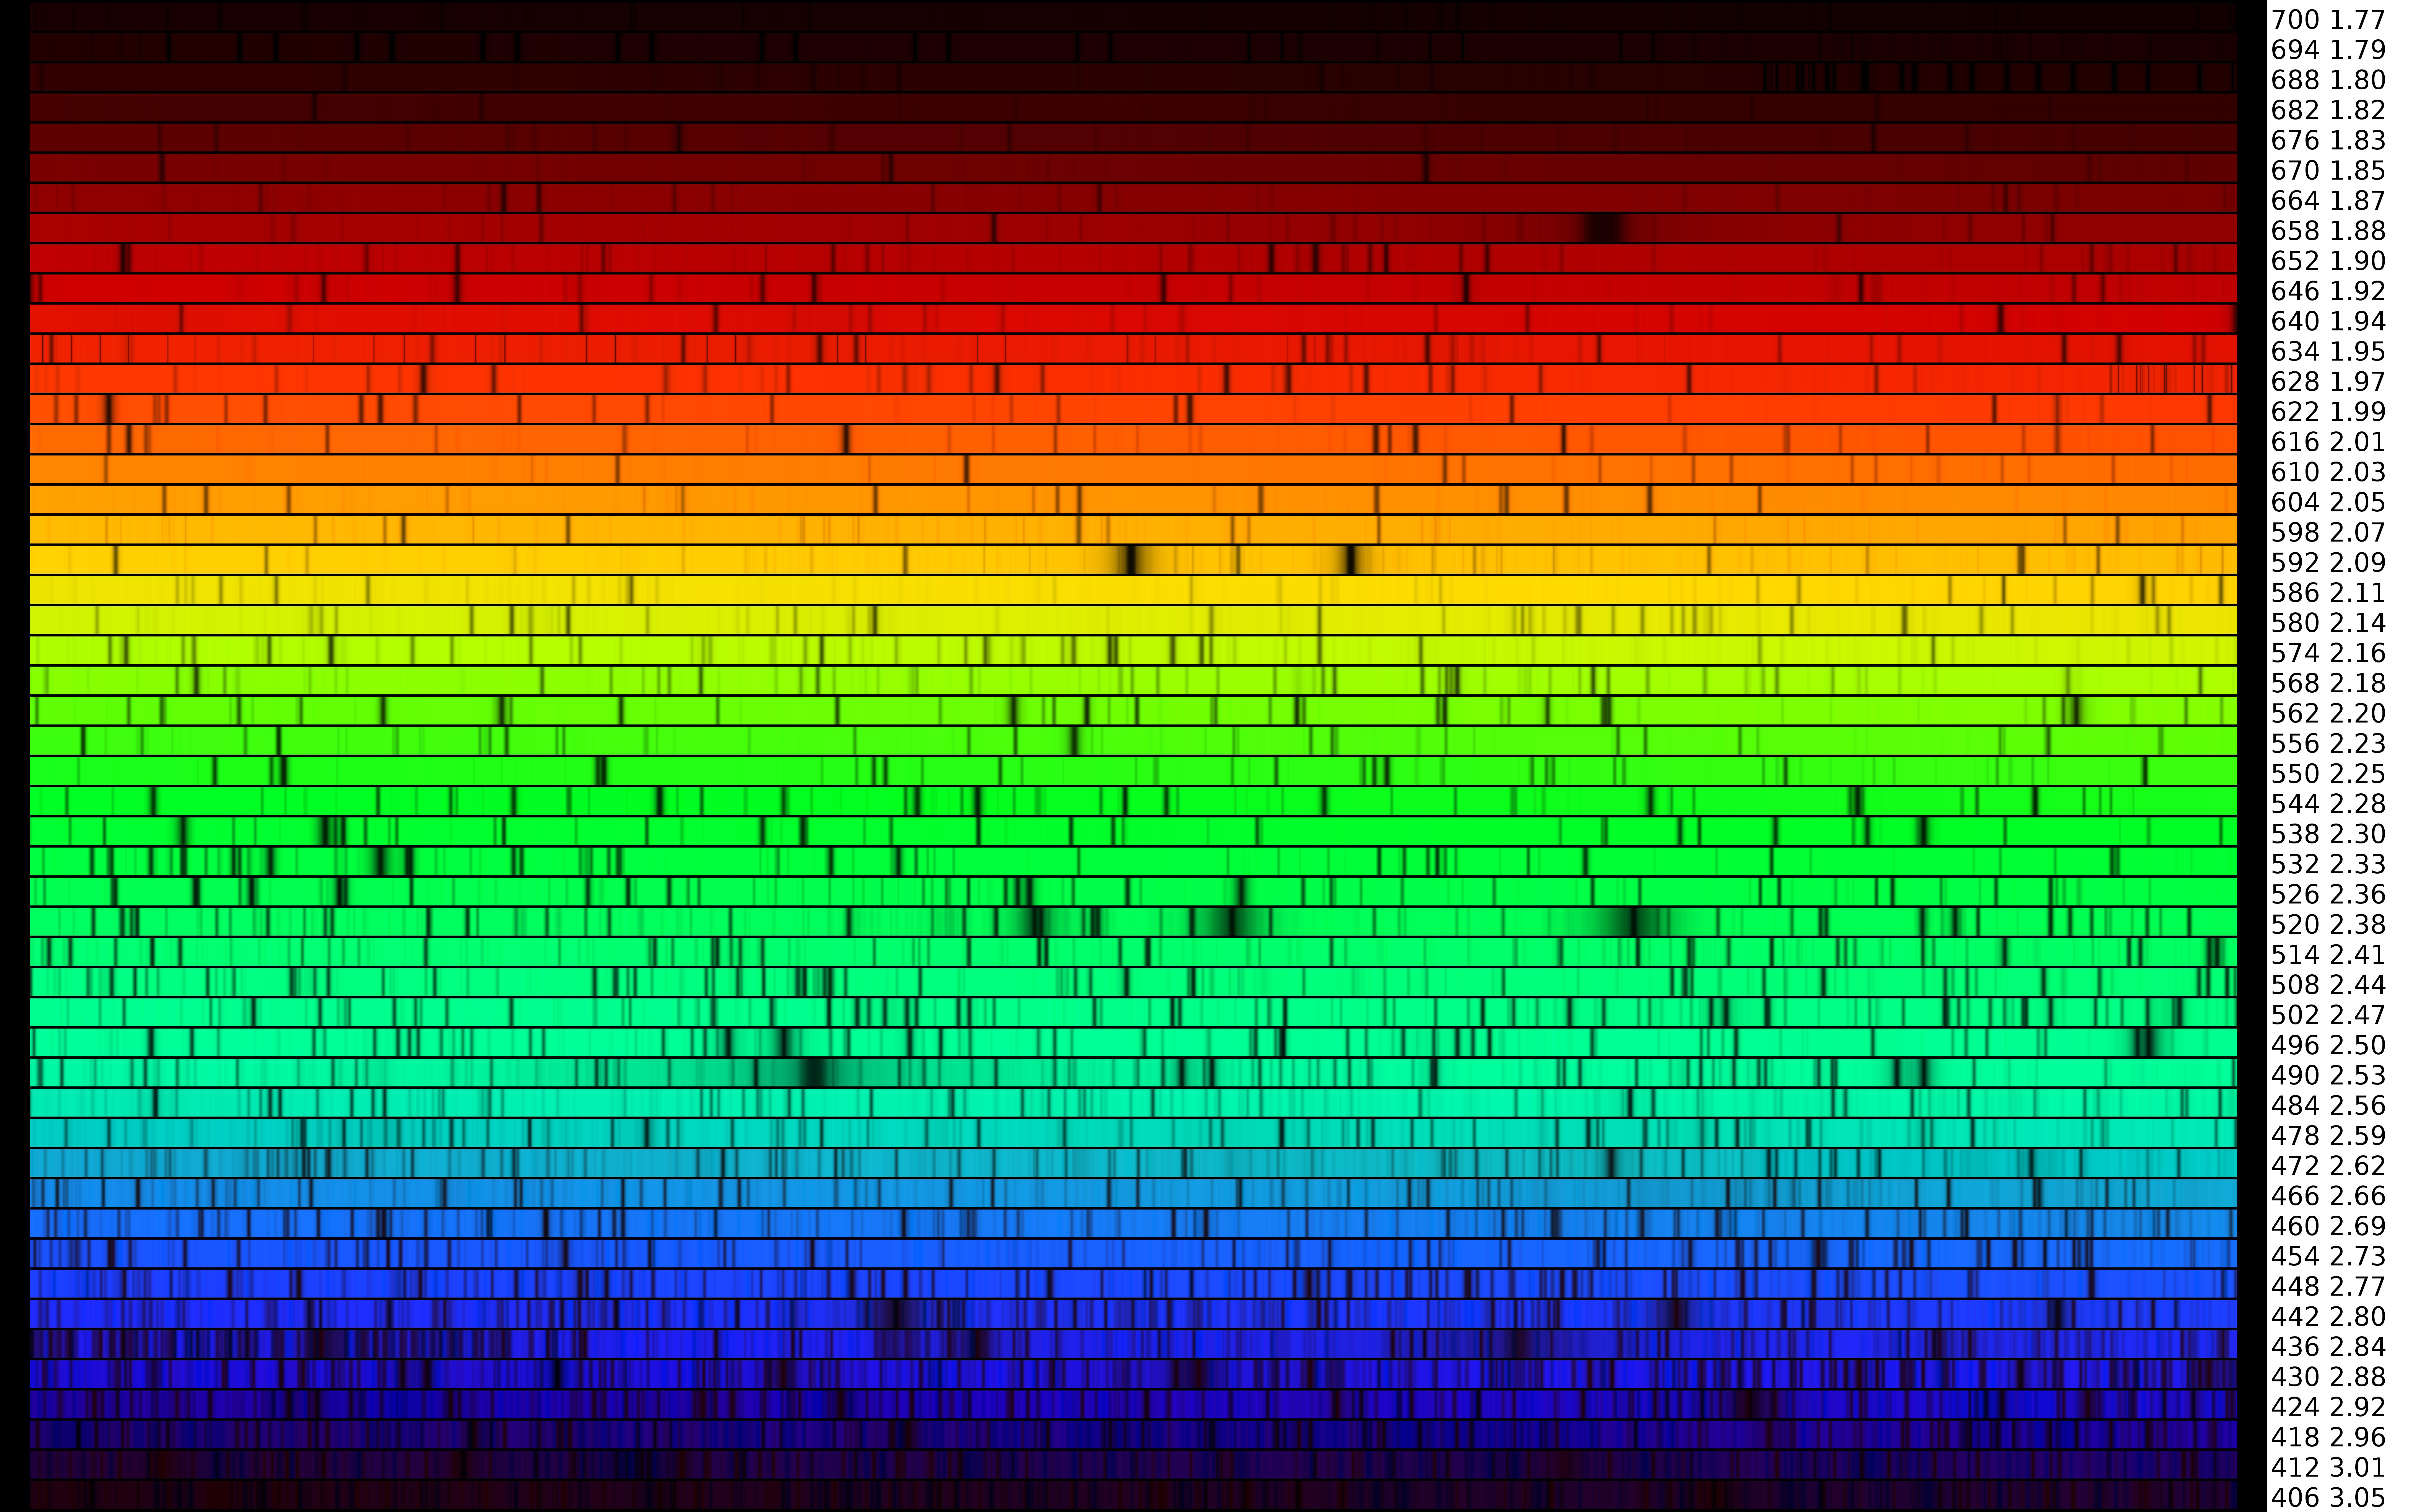
\includegraphics[width=\textwidth]{solarspectrum.jpg}\EC
}

\frame{\frametitle{\textbf{Announcements}}
\large
\BI
\item Paper due Nov 3 (not Nov 1)
\BS

\item A few of our coaches have offered to help people with paper drafts:
\BI
\item Kiersten Edwards - kedwar03@syr.edu
\item Xinning Li - xli287@syr.edu (bilingual in English and Chinese)
\EI
\EI
}

\frame{\frametitle{\textbf{Announcements}}
	\large
	Slight modification to the planned homework schedule:
	\BI
	\item Just one homework assignment this unit
	\item It will be assigned Thursday (next class)
	\item It will be due the following Thursday
	\item We'll have time for questions, plus a quiz that day 
	\pause
	\item (This is also the new date your papers are due -- don't do everything at the last minute!)
\EI
}


\frame{\frametitle{\textbf{Exam 2 retrospective}}
	\large
	Confession time:
	\BI
	\item Exam 2 was so mewhat more difficult than I meant for it to be\pause
	\item This is because I didn't get as much time to write it as usual\pause
	\BS
	\item We still think this did a reasonably decent job being ``fair'' -- it was just a bit too hard \pause
	\BS
	\item We're going to rescale the grades to reflect this
	\BI
	\item Your letter grade will thus be higher than what's written on your exam
	\item It will also be worth slightly less
	\EI
	\EI
}


\frame{\frametitle{\textbf{The quantum nature of light}}
	
	\Large \BC Light has both particle properties and wave properties:\EC
	
	
	\normalsize
	\BI
	\item Particle properties: it comes in discrete chunks called {\it photons}, each carrying a certain {\color{Green}energy}.
	\item Wave properties: it has a {\color{Red} wavelength} $\lambda$ and {\color{Red} frequency} $f$ 
	\EI
	
	\BS\BS
	
	We thus have three ways to distinguish different colors:
	
	\BS
	
	
	{\color{A} ``Redder'' colors (red, infrared, microwave, radio) have:
		\BI
		\color{A}
		\item Longer wavelengths
		\item Less energy per photon 
		\item Lower frequencies (we usually don't care)
		\EI
	}

	
{\color{D} ``Bluer'' colors (blue, ultraviolet, x-rays, gamma rays) have:
	\BI
	\color{D}
	
	\item Shorter wavelengths
	\item More energy per photon 
	\item Higher frequencies (we don't care)
	\EI
}
}
	
	
	
	
	

\frame{
	
	\BC
	\Large
	We have lots of names for different sorts of light.
	
	\BS
	
	They differ only in wavelength/energy/frequency, and the other things they interact with.
	\EC
	
	\large
	\BI
	\item Radio waves: used to communicate over long distances
	
	\BS
	
	\item Microwaves: used to communicate over short distances
	
	\BS
	
	\item ``Far infrared'': associated with objects with temperatures close to ours
	
	\BS
	
	\item ``Near infrared'': much like light, but we can't see it
	
	\BS
	
	\item Visible light (only a very narrow range!)
	
	\BS
	
	\item Ultraviolet: enough energy to disrupt atoms
	
	\BS
	
	\item X-rays: enough energy to penetrate human tissue
	
	\BS
	
	\item Gamma rays: enough energy to disrupt atomic nuclei!
	
	\BS
	
	\EI
	
}


\frame{\frametitle{\textbf{Types of light}}
	
	As you go down the table:
	
	\begin{itemize}
		\item Wavelength decreases
		\item Frequency increases (not shown)
		\item Energy per photon increases
		\pause
		\item These are just names -- all light is really the same kind of thing
	\end{itemize}
	
	\scriptsize
	\begin{table}[]
		\begin{tabular}{|l|l|l|l|}
			\hline
			& Wavelength             & Energy                   & Application                   \\ \hline
			Radio waves         & 100 meters - 1 meter   &                          & Long distance communication   \\ \hline
			Microwaves          & 1 meter - 1 cm         & Too small to matter      & Short distance communication  \\ \hline
			"Far infrared"      & 1 cm - 10 $\mu$m      & Thousandths of an eV     & Radiated by room temp objects \\ \hline
			"Near infrared"     & 750 nm - 10000 nm      & Tenths of an eV - 1.6 eV & ``Invisible light"             \\ \hline
			Visible light       & 380-750 nm             & 1.6 eV - 3.2 eV          & Eyeballs!                     \\ \hline
			Near ultraviolet    & 100-380 nm             & 3.2 eV - 10 eV           & ``Invisible light"             \\ \hline \color{Red}
			Extreme ultraviolet & 1 nm - 100 nm          & \color{Red}10 eV - 1000 eV          & Etching computer chips        \\ \hline
			\color{Red}X-rays              & Trillionths of a meter & \color{Red}1000 eV - 1 million eV   & Medical imaging               \\ \hline
			\color{Red}Gamma rays          & Too small to matter      & \color{Red}Millions of eV           & Nuclear transitions           \\ \hline
		\end{tabular}
	\end{table}
	
}

\frame{
	
	\BC
	\Large All of these are ``types of light''. 
	
	\BS
	
	They differ only in wavelength/frequency/energy!
	
	\BS\BS
	
	\includegraphics[width=\textwidth]{EMSpec.png}
	\EC
}



%
%\frame{
%	\Huge\BC
%	\it At what point does spaghettification occur? \rm
%	
%	\bigskip
%	\huge\begin{flushright}--Harris Krahn\end{flushright}
%	\EC
%}

\frame{
	
	\Large
	
	Lots of folks are curious about different types of ``radiation'' -- in particular, how it can affect human health.

\bigskip
	
	Do you have any questions about this?
	\bigskip
	\begin{center}
	\includegraphics[width=0.96\textwidth]{EMSpec.png}	
	\end{center}
}

\frame{\frametitle{\bf Light and spectra}

\Large\BC

White light isn't really white; it's a mix of many colors (wavelengths).

\BS

Our eyes are very limited; we can only distinguish between three colors.

\BS

We can learn a lot about an object by the colors of light it emits, but we have to be able to see them first!

\BS

We do that by spreading them out. Then we can see what colors are there in great detail.
\EC
}

\frame{
\BC
\Large
A friend sent me this a few years ago, the day before we did this topic:

\BS

\includegraphics[width=0.4\textwidth]{text.png}
\EC

}

\frame{


\BC
\Large
The two pictures:

\BCC
\HC\BC
\Large Shortly after sunrise:

\includegraphics[width=0.6\textwidth]{spectrum-blue-deficit.jpg}
\EC
\HC\BC
\Large Later in the day:

\includegraphics[width=0.6\textwidth]{spectrum-normal.jpg}
\EC

\ECC
\pause\BS

\Large What is different?
\EC
}

\frame{

\BC
\Huge
What happened here?
\EC
\Large
\BS
\color{A}A: There's less blue light right after sunrise because the Sun is different then\\ \medskip
\color{B}B: The colors are in a different order earlier in the day\\ \medskip
\color{C}C: All the colors are fainter right after sunrise\\ \medskip
\color{D}D: There's less blue light right after sunrise because something happened to the light as it was traveling here\\

}

\frame{
\Large
\BC
Let's look at that picture of the Sun again:

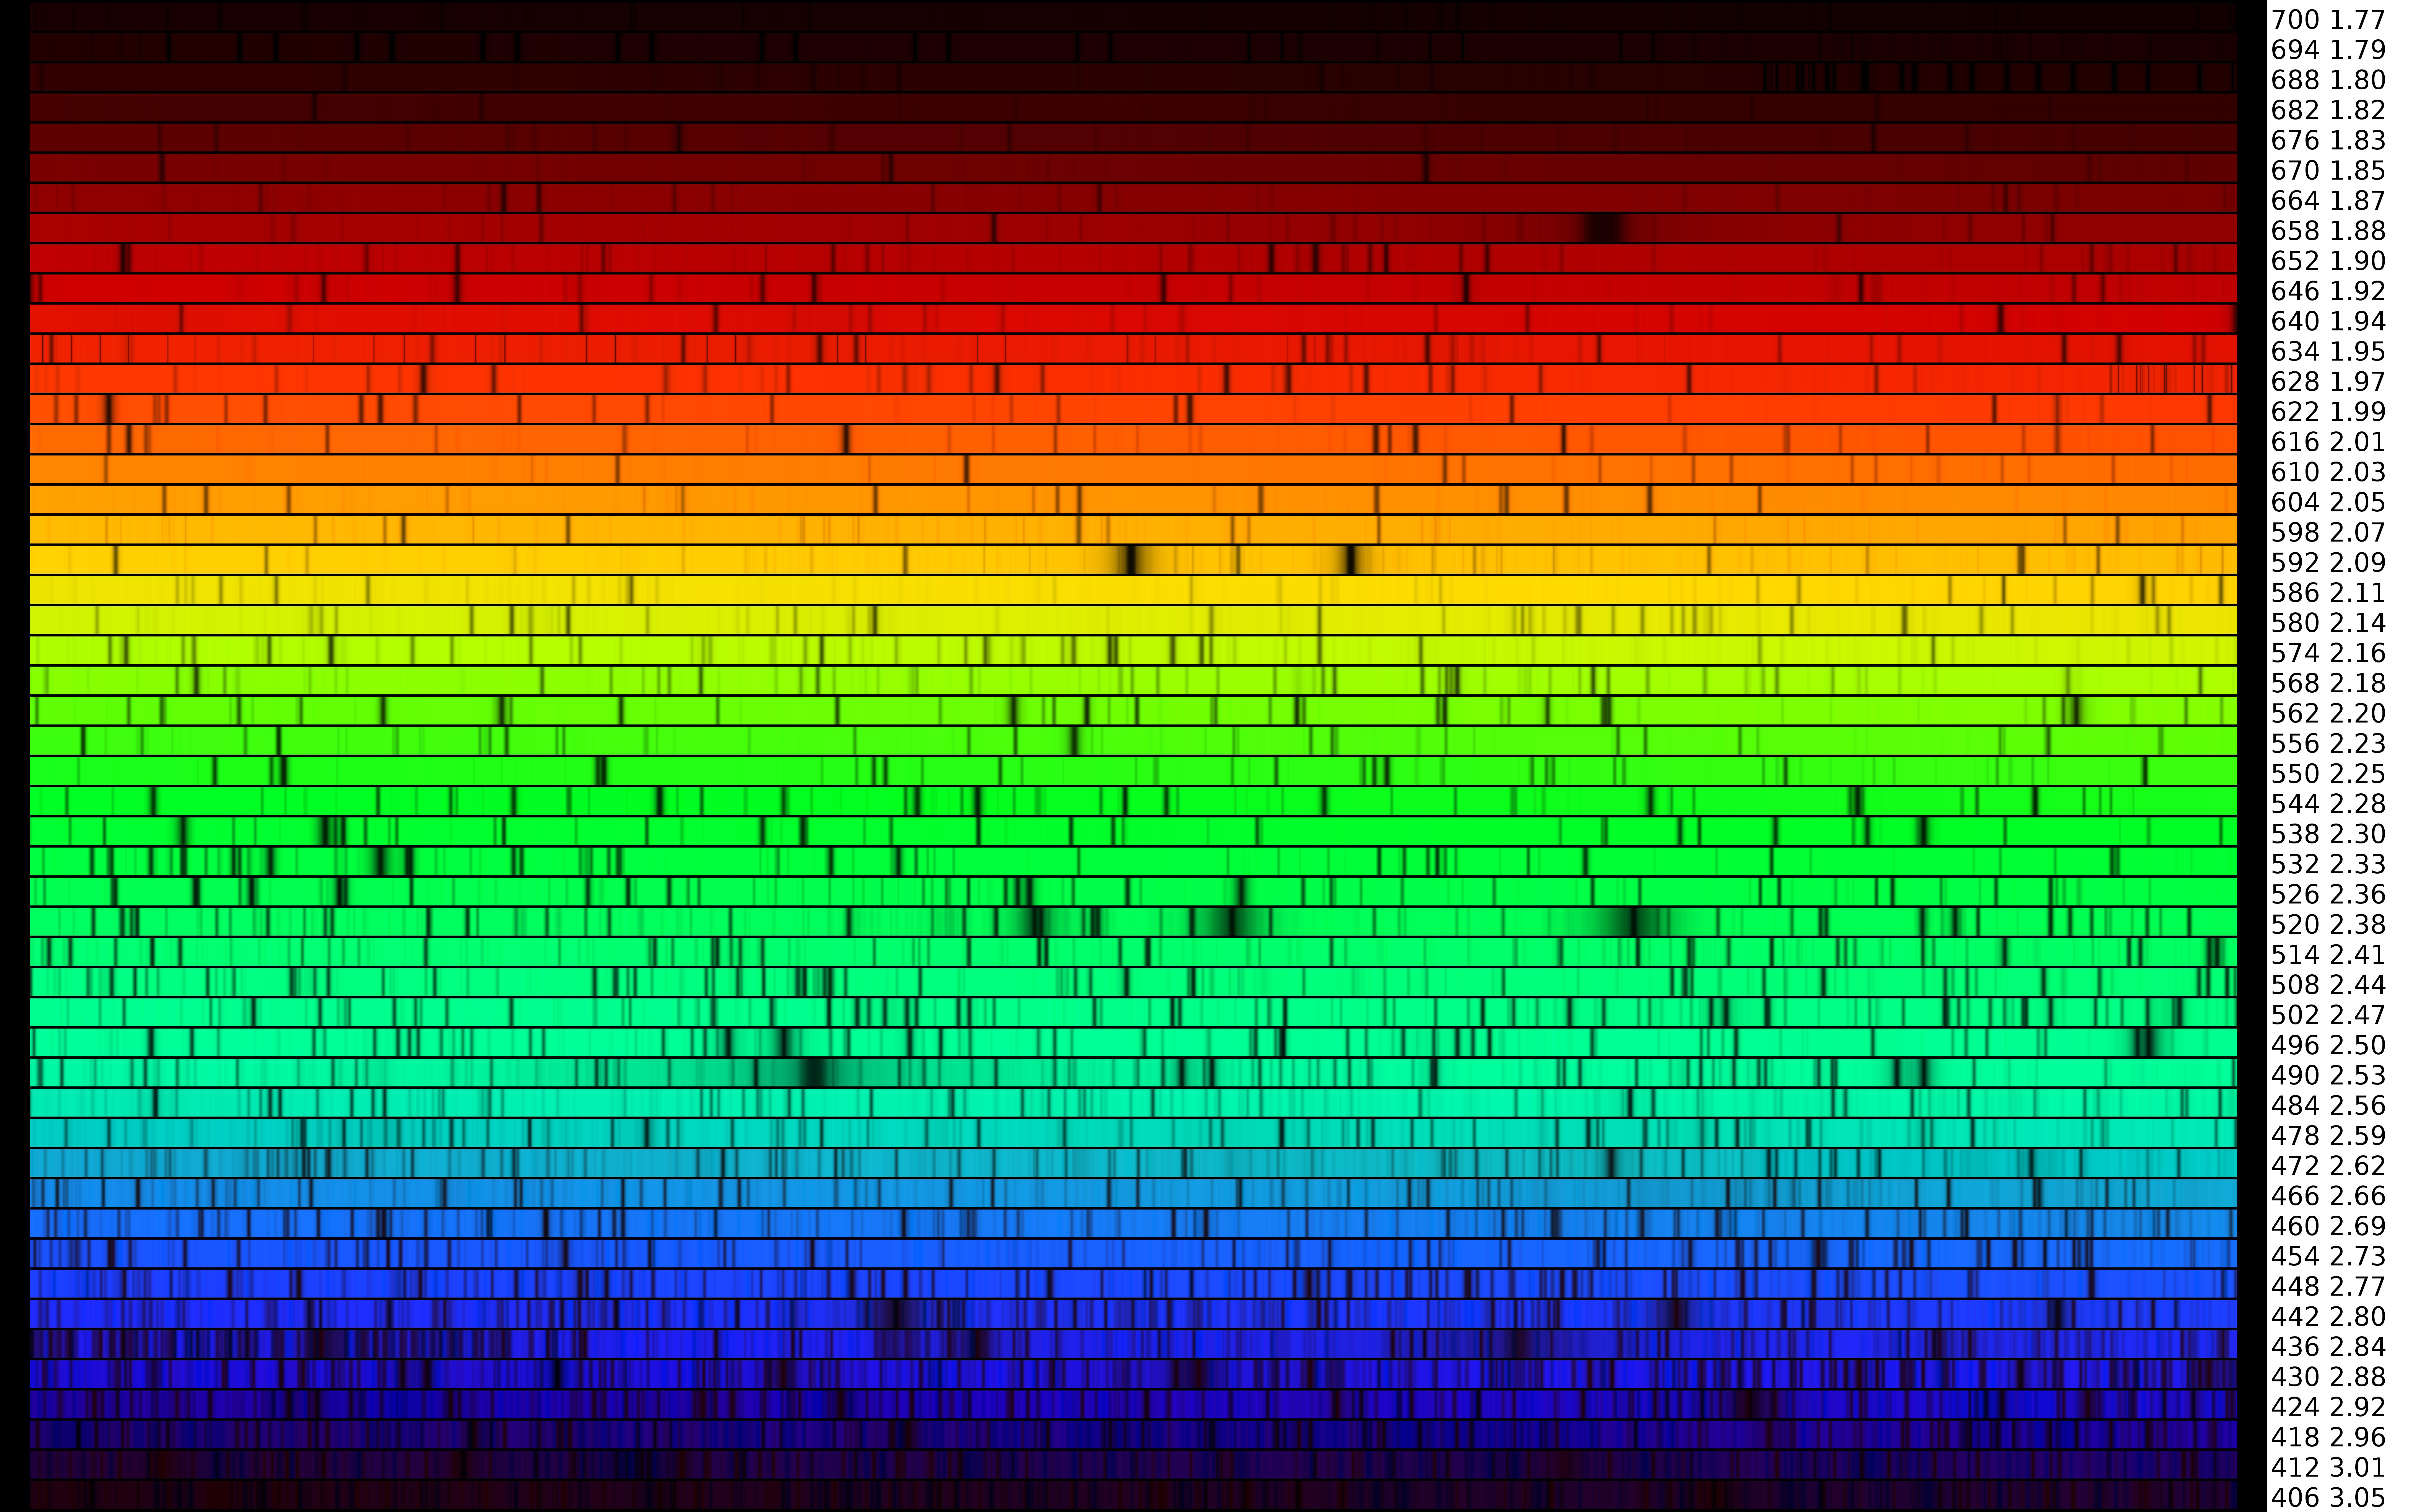
\includegraphics[width=0.7\textwidth]{solarspectrum.jpg}

\pause
\large
Need to understand:
\BI
\item Where did all those colors come from in the first place? (today)
\item What can we learn about the sizes and temperatures of stars by their colors (next Tuesday)
\item Why are there dark lines? (next Thursday)
\EI
\EC
}

\frame{
\Huge
\BC
Why does the sun shine?
\EC
\BS

\color{A}A: Chemical reactions make light! \\
\color{B}B: Nuclear reactions make light! \\
\color{C}C: It's really hot, so it glows \\
\color{D}D: That's just what stars do \\
\pause
\color{E}E: Google to the rescue!
}


\frame{\frametitle{\textbf{Incandescence}}
\large

``The sun is a mass of incandescent gas'' -- what does that mean?

\BC
\Large
{\color{Red}Objects glow because they're hot. This is called {\it thermal radiation}.}
\EC
\BS
\BS
\normalsize
\BI
\item Any object with a temperature emits electromagnetic radiation (``light'').
\item For objects as warm as we are, this is in the ``far infrared''.
\item As objects heat up, the peak wavelength decreases (the average photon energy increases)
\item As objects heat up, the total intensity emitted goes up {\it rapidly} (proportional to $T^4$)
\item This is also called ``blackbody radiation'' (since even a black object glows if it's warmed up)
\EI

\BS
\BC
See the simulation to see how this works...
\EC
}

\frame{\frametitle{\textbf{Takeaways: thermal radiation}}

\Large

\BI
\item Any object with a temperature glows
\item Hotter objects glow ``bluer'' (shorter wavelengths) and brighter
\item Hotter objects emit more light per unit area (of all wavelengths)
\item A larger object that is cold (large red star) may emit more total light than a small object that is hot (small yellow star)
\item This glow is a {\it broad spread of wavelengths} -- there aren't narrow bright or dark lines in it
\EI
}


\frame{
\Large
What will happen if I turn the power up on the lamp?

\BS\BS

\color{A}A: The height of the graph will go up \\
\color{B}B: The graph will shift left \\
\color{C}C: The graph will shift right \\
\color{D}D: The height of the graph will go down \\
}



\frame{\frametitle{\textbf{Another table}}

\Large

It's important to know, roughly, what temperature objects emit radiation of what wavelengths (mostly):


\footnotesize
\bigskip
\bigskip

\begin{tabular}{|l|l|l|l|}

\hline

Name             & Temp (Kelvin)     & Temp (Celsius)    & Object                               \\ \hline
Microwaves       & 3                 & -270              & The universe itself                  \\ \hline
Infrared         & 300               & 30                & Stuff on Earth                       \\ \hline
Near infrared    & 1500              & 1200              & A candle flame (mostly IR, some red) \\ \hline
Visible (middle) & 5000              & 5000              & A star like the Sun                  \\ \hline
Ultraviolet      & Tens of thousands & Tens of thousands & A very hot star, like Rigel          \\ \hline
X-ray            & Millions          & Millions          & Gas falling into a black hole        \\ \hline
\end{tabular}
}

\frame{
	
	\huge
	
	\BC
	Let's practice this.
	
	\large
	
	This sort of thing will be on your homework (assigned Thursday) and on the following homework quiz.
	\EC
}


%
%\frame{
%\Large
%What will happen if I put a colored plate in between?
%
%\BS\BS
%
%\color{A}A: The height of the graph will go down \\
%\color{B}B: A narrow dip will appear in the graph \\
%\color{C}C: A narrow peak will appear in the graph \\
%\color{D}D: The graph will shift left \\
%\color{E}E: The graph will shift right 
%}




\frame{

\BC
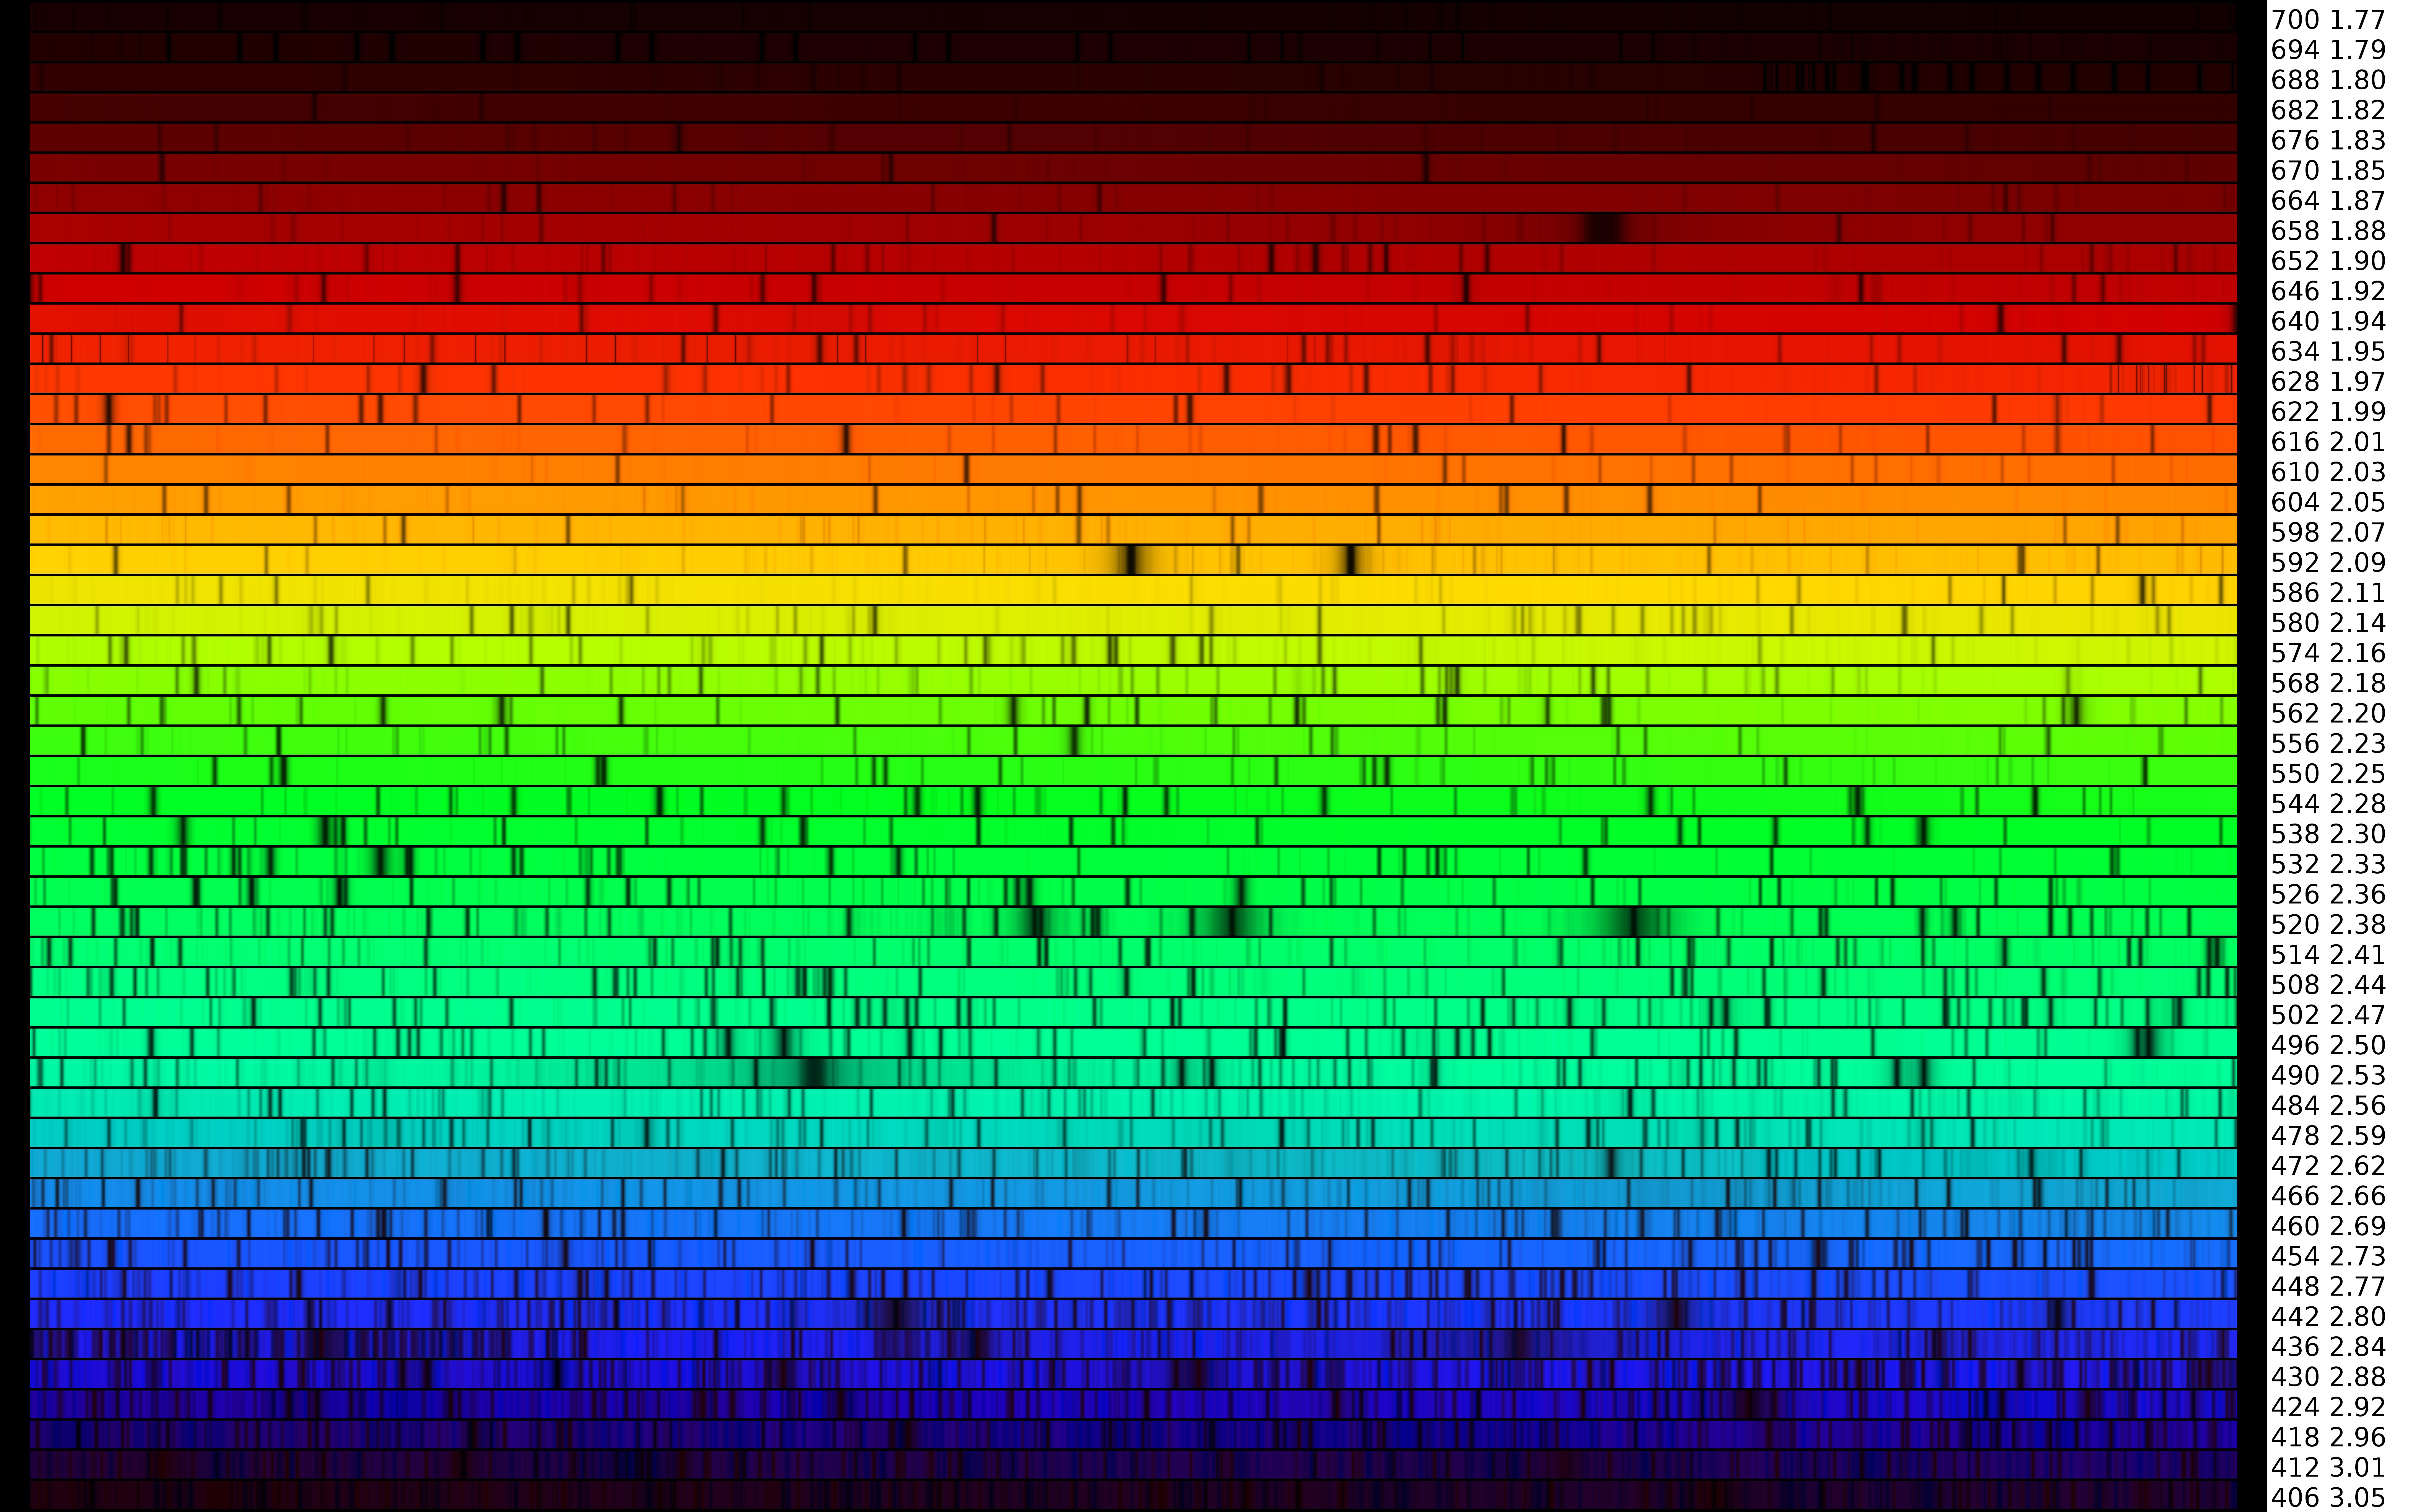
\includegraphics[width=0.7\textwidth]{solarspectrum.jpg}
\EC

\BI
\item The hot core of the Sun emits light of all wavelengths 
\pause
\item The gases in the cooler atmosphere absorb very particular colors ... but why, and which ones? 
\EI
}

%\frame{\frametitle{\textbf{Chemistry 101 in a nutshell}}
%\Large
%\BC
%(on the document camera)
%\EC
%}
%
%\frame{
%\Huge\BC
%Start on {\it Lecture Tutorials} pp. 65-69.
%
%\BS
%\large
%
%This is the crux of this unit, so ask lots of questions to us!
%\EC
%}

\end{document}
